\chapter{Introduction}

Cities are a central feature of human society - Human beings are increasingly an urban species. Cities are one of the primary sources of technological development and increasing wealth. Behind these observations is a fundamental feature demonstrated in the recent literature on scaling laws: the productivity of cities increases super-linearly in population. Cities are the locus of a positive feedback loop: rising populations raises productivity, rising productivity attracts more people and resource.

Cities are where people live and work, where a great deal of production is concentrated, in addition to being where wealth is created and accumulated, cities are also where income is actually distributed. 

In Canada, there is a housing crisis. In the last few years, the need for affordable housing has come into focus as one of the most pressing issues facing Canadians. As more and more Canadians are finding housing unaffordable, the effects are being seen in everything from declining home ownership rates to an increasing number of Canadians unable to afford housing at all.

There has been extensive work on the drivers of the crisis, including supply shortages, stagnating incomes, and the finacialization of housing ownership.

There has been less work on the implications for productivity. The housing crisis raises the question of whether Canadian cities can continue to attract people and accumulate wealth for its residents and industries, whether in fact it can even sustain their growth.

This thesis presents a spatial model of the city that incorporates distributional issues and financialization and allows us to examine the productivity implications of the housing crisis. The model that incorporates the scaling of productivity in cities within a standard urban model. 
The urban model is based on those developed in geography, planning and urban economics. The organizing principle in  the spatial models of all three disciplines is an economic variable, land rent, which is the link to distribution, financialization and continuing productivity. *** (another sentence on why this is great)

The analysis makes clear that in addition to the recognized distributional consequences, the housing crisis has productivity impacts that should be considered in developing urban and housing policy. Sopecifically, the analysis in this thesis concludes that, given the ongoing financialization of the housing market,


\begin{enumerate}
\item the financial system will eventually extract all net urban land rents through investment in urban property
\item housing accessibility will become increasingly challenging for disadvantaged groups
\item housing will be largely eliminated as a saving mechanism and asset fr middle income Canadians,  resulting in a systematic decline in the `middle class'
\item that the quality of urban life will decline
\item the economic growth and development of cities is threatened by this financialization
\end{enumerate}


The focus of this thesis on a topic. that falls in the overlap  between least three academic  disciplines, Economics, Urban Geography, and Planning. The central and shared concern in this area is with geographic space.



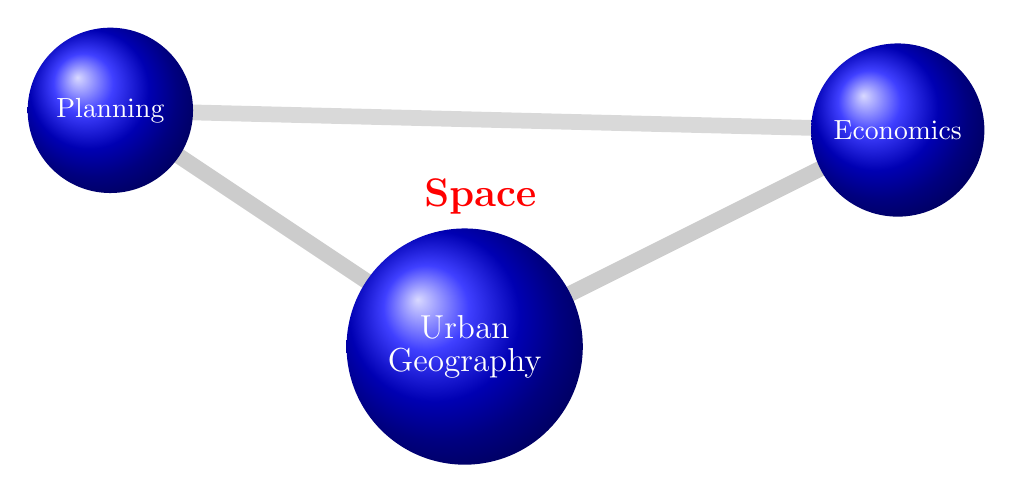
\begin{tikzpicture}{scale=.5}
% find color cotrol for ball. Tind way to stop line short of node
\coordinate (planning) at (-5,1);%PREFACE
\coordinate (economics) at (5,.75);%
 \coordinate (geography) at (-.5,-2); %history
\coordinate (finance) at (0,5); %

\draw [line width=2mm, black!15, ] (planning)--(economics);
\draw [line width=2mm, black!20, ] (geography)--(economics);
\draw [line width=2mm, black!20, ] (geography)--(planning);

%\draw [line width=2mm, black!25, ] (geography)--(finance);
%\draw [line width=2mm, black!20, ] (planning)--(finance);
%\draw [line width=2mm, black!20, ] (finance)--(economics);

\node [circle,shading=ball, minimum width=2.1   cm, white, align=center] (ball) at (planning) {Planning};
\node [circle,shading=ball, minimum width=2.2cm, white, align=center] (ball) at (economics) {Economics};
\node [circle,shading=ball, minimum width=3 . cm, white, align=center] (ball) at (geography)[text width=2cm] {\large Urban\\ Geography};

%\node [circle, shading=ball, minimum width=2.4cm, white, align=center] (ball) at (finance)[text width=2cm] {Finance};

\node at (-.3,-.1) [red] {\Large \textbf{Space}};
\end{tikzpicture}

Figure 1: The common concern of three fields
topic 

A simple economic insight -- that locational value gives rise to land rents -- provides an organizing principle for the three disciplines. Rent theory has a long history in economics, going back to thinkers such as Richard Cantillon (1680s-1734), François Quesnay (1694–1774), the marquis de Mirabeau (1715–1789) and Anne-Robert-Jacques Turgot (name physiocrat) and Adam Smith (1723-1790) and received its classic statement in Ricardo (1772-1823). Nearly contemporaneous thinker, Johann Heinrich  von Th\"unen (1783-1850) developed a planning model to guide the location of economic activities for an urban-agricultural society.  A version of that model  was reinvented in urban geography by XXX. Alonzo\footnote{We use a version of the well-established model of Alonso (1964), Muth (1969) and Mills (1967), and formalised by Wheaton (1974),}

We link the Alonzo model with more recent work on growth theory starting with Robert Solo's XXX and with the endogenous growth models of Lucas () and draw on Jane Jacobs's insight that endogenous urban growth  is. now driving economic development. Jacobs's insight is empirically supported by recent work in the complexity literature on urban scaling by XXXX ()




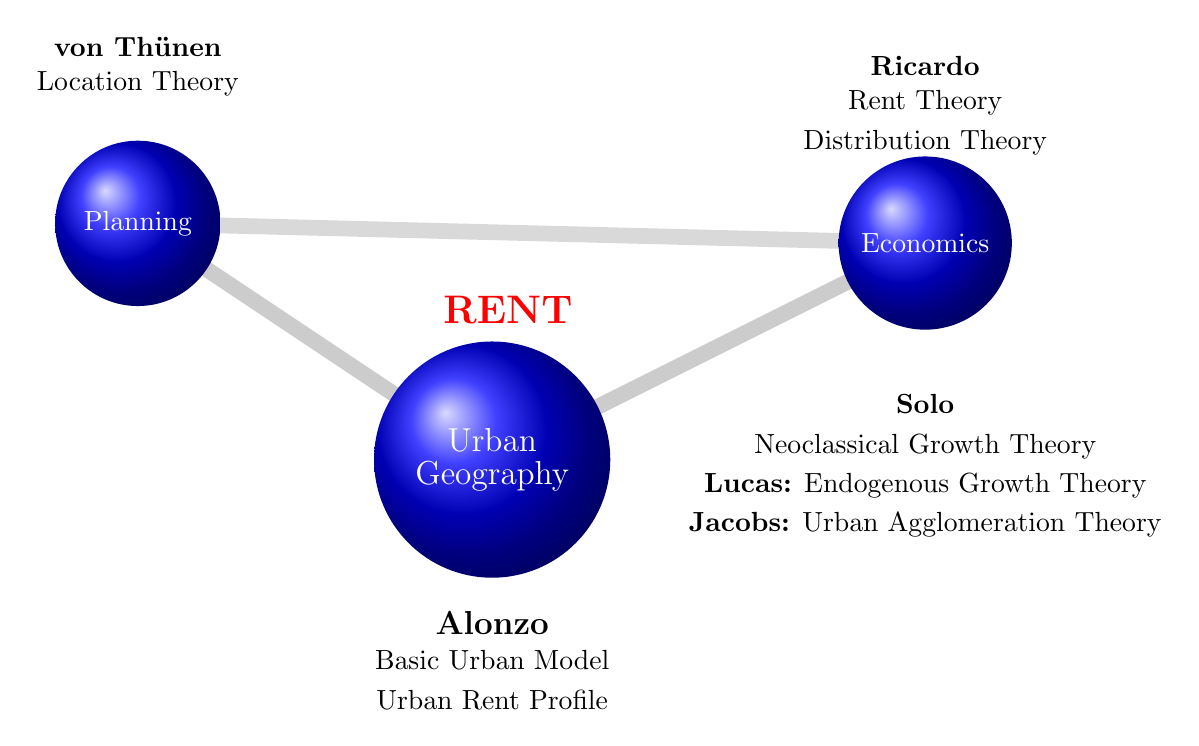
\begin{tikzpicture}{scale=.5}
% find color cotrol for ball. Tind way to stop line short of node
\coordinate (planning) at (-5,1);%PREFACE
\coordinate (economics) at (5,.75);%
 \coordinate (geography) at (-.5,-2); %history
\coordinate (finance) at (0,5); %

\draw [line width=2mm, black!15, ] (planning)--(economics);
\draw [line width=2mm, black!20, ] (geography)--(economics);
\draw [line width=2mm, black!20, ] (geography)--(planning);

%\draw [line width=2mm, black!25, ] (geography)--(finance);
%\draw [line width=2mm, black!20, ] (planning)--(finance);
%\draw [line width=2mm, black!20, ] (finance)--(economics);

\node [circle,shading=ball, minimum width=2.1   cm, white, align=center] (ball) at (planning) {Planning};
\node [circle,shading=ball, minimum width=2.2cm, white, align=center] (ball) at (economics) {Economics};
\node [circle,shading=ball, minimum width=3 . cm, white, align=center] (ball) at (geography)[text width=2cm] {\large Urban\\ Geography};

%\node [circle, shading=ball, minimum width=2.4cm, white, align=center] (ball) at (finance)[text width=2cm] {Finance};

\node at (-.3,-.1) [red] {\Large \textbf{RENT}};

% new stuff
\node at (planning) [above=2cm] {\textbf{von Th\"unen}};
\node at (planning) [above=1.5cm] {Location Theory};

\node at (economics) [above=2cm] {\textbf{Ricardo}};
\node at (economics) [above=1.5cm] {Rent Theory};
\node at (economics) [above=1.0cm] {Distribution Theory};

\node at (economics) [below=1.8cm] {\textbf{Solo}};
\node at (economics) [below=2.3cm] {Neoclassical Growth Theory};
\node at (economics) [below=2.8cm] {\textbf{Lucas:} Endogenous Growth Theory};
\node at (economics) [below=3.3cm] {\textbf{Jacobs:} Urban Agglomeration Theory};


\node at (geography) [below=1.8cm] {\textbf{\large Alonzo}};
\node at (geography) [below=2.3cm] {Basic Urban Model};
\node at (geography) [below=2.8cm] {Urban Rent Profile};
\end{tikzpicture}

Figure 3: space and value

Land rent was historically the basis of the wealth and political power of  the land-owning class in the era of the classical economists.


We further link the model of urban rents to emerging concerns about the financialization of the housing market. The key insight we offer is that the financialization  of the housing sector is a  form of rent-seeking that must have detrimental effects on urban development and on the well-being of urban residents.





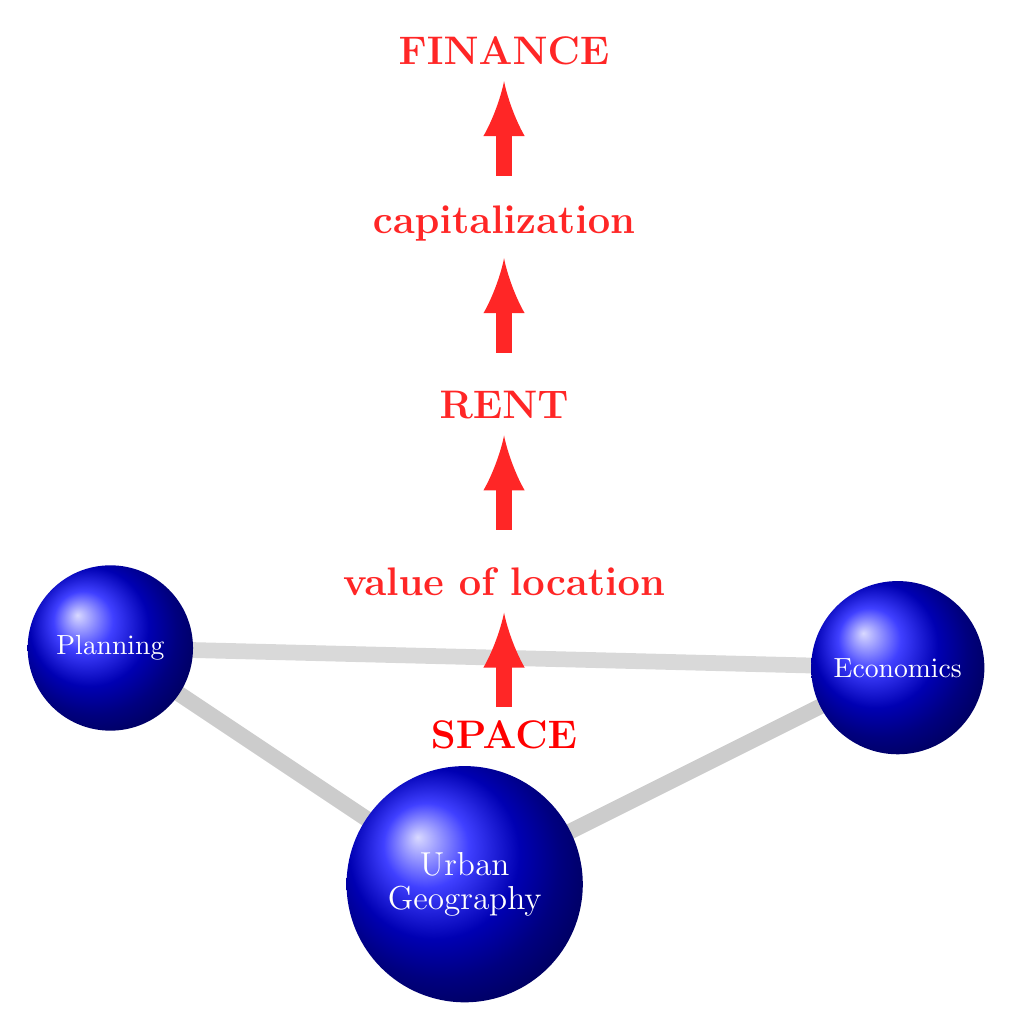
\begin{tikzpicture}{scale=.5}
% find color cotrol for ball. Tind way to stop line short of node
\coordinate (planning) at (-5,1);%PREFACE
\coordinate (economics) at (5,.75);%
 \coordinate (geography) at (-.5,-2); %history
\coordinate (finance) at (0,5); %

\draw [line width=2mm, black!15, ] (planning)--(economics);
\draw [line width=2mm, black!20, ] (geography)--(economics);
\draw [line width=2mm, black!20, ] (geography)--(planning);

%\draw [line width=2mm, black!25, ] (geography)--(finance);
%\draw [line width=2mm, black!20, ] (planning)--(finance);
%\draw [line width=2mm, black!20, ] (finance)--(economics);

\node [circle,shading=ball, minimum width=2.1   cm, white, align=center] (ball) at (planning) {Planning};
\node [circle,shading=ball, minimum width=2.2cm, white, align=center] (ball) at (economics) {Economics};
\node [circle,shading=ball, minimum width=3 . cm, white, align=center] (ball) at (geography)[text width=2cm] {\large Urban\\ Geography};

%\node [circle, shading=ball, minimum width=2.4cm, white, align=center] (ball) at (finance)[text width=2cm] {Finance};
\draw [line width=2mm, red!85, -latex ] (0, 7)--++(0,1.2)node[above=-.1] {\Large \textbf{FINANCE}};
\draw [line width=2mm, red!85, -latex ] (0, 4.75)--++(0,1.2)node[above=-.1] {\Large \textbf{capitalization}};
\draw [line width=2mm, red!85, -latex ] (0, 2.5)--++(0,1.2)node[above=-.1] {\Large \textbf{RENT}};
\draw [line width=2mm, red!85, -latex ] (0, .25)--++(0,1.2)node[above=-.1] {\Large \textbf{value of location}};
\node at (0,-.1) [red] {\Large \textbf{SPACE}};
\end{tikzpicture}



% \vspace {2cm}
% Figure 4 with finance

% \begin{tikzpicture}{scale=.5}
% % find color cotrol for ball. Tind way to stop line short of node
% \coordinate (planning) at (-5,1);%PREFACE
% \coordinate (economics) at (5,.75);%
%  \coordinate (geography) at (-.5,-2); %history
% \coordinate (finance) at (0,5); %

% \draw [line width=2mm, black!15, ] (planning)--(economics);
% \draw [line width=2mm, black!20, ] (geography)--(economics);
% \draw [line width=2mm, black!20, ] (geography)--(planning);

% \node at (-.3,2) [red] {\huge \textbf{RENT}};

% \draw [line width=3mm,  black!50,opacity=.5 ] (geography)--(finance);
% \draw [line width=2mm, black!20, ] (planning)--(finance);
% \draw [line width=2mm, black!20, ] (finance)--(economics);

% \node [circle,shading=ball, minimum width=2.1   cm, white, align=center] (ball) at (planning) {Planning};
% \node [circle,shading=ball, minimum width=2.2cm, white, align=center] (ball) at (economics) {Economics};
% \node [circle,shading=ball, minimum width=3 . cm, white, align=center] (ball) at (geography)[text width=2cm] {\large Urban\\ Geography};

% \node [circle, shading=ball, minimum width=2.4cm, white, align=center] (ball) at (finance)[text width=2cm] {Finance};


% \end{tikzpicture}

Summarizing the overall focus of the thesis,  we are concerned with the implication for urban development of growing rent extraction by the financial sector.  

\vspace {2cm}
Figure 4 with finance

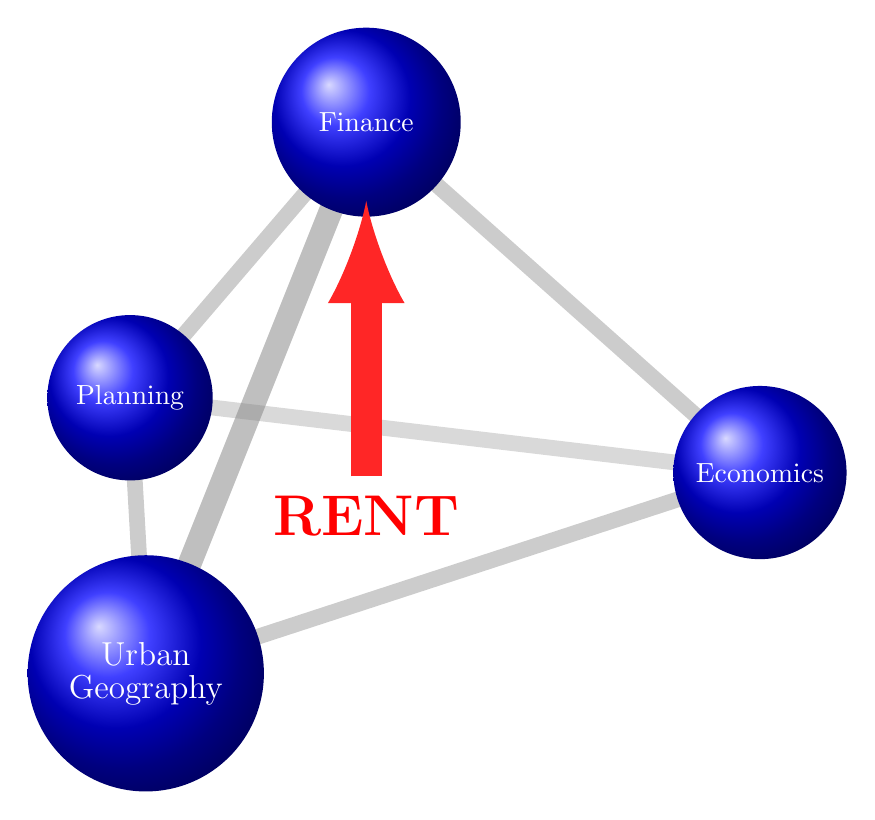
\begin{tikzpicture}{scale=.5}
% find color cotrol for ball. Tind way to stop line short of node
\coordinate (planning) at (-3,1.5);%PREFACE
\coordinate (economics) at (5,.55);%
 \coordinate (geography) at (-2.8,-2); %history
\coordinate (finance) at (0,5); %

\draw [line width=2mm, black!15, ] (planning)--(economics);
\draw [line width=2mm, black!20, ] (geography)--(economics);
\draw [line width=2mm, black!20, ] (geography)--(planning);

\node at (.0,0) [red] {\huge \textbf{RENT}};

\draw [line width=3mm,  black!50,opacity=.5 ] (geography)--(finance);
\draw [line width=2mm, black!20, ] (planning)--(finance);
\draw [line width=2mm, black!20, ] (finance)--(economics);

\node [circle,shading=ball, minimum width=2.1   cm, white, align=center] (ball) at (planning) {Planning};
\node [circle,shading=ball, minimum width=2.2cm, white, align=center] (ball) at (economics) {Economics};
\node [circle,shading=ball, minimum width=3 . cm, white, align=center] (ball) at (geography)[text width=2cm] {\large Urban\\ Geography};

\node [circle, shading=ball, minimum width=2.4cm, white, align=center] (ball) at (finance)[text width=2cm] {Finance};
\draw [line width=4mm, red!85, -latex ] (0, .5)--(0,4);


\end{tikzpicture}



\section{Document Overview}

\textbf{In chapter XXX}  we link classical rent theory, neoclassical production theory, neoclassical growth theory, the scaling literature, and urban spatial models.
To show how our model is directly connected with this broad collection of linked theories, we use the Cobb-Douglas function, which is used across this entire range of literature 

After we develop the mathematical description of the relationship among these will discuss  in more detail, rent theory and our contribution, scaling laws, ......  and other issues in the literature that draw on parts of this model and 

???  apply to the specific situation we're in why rent theory is related to discussions of exploitation why it might lead the inefficiencies, whether or not this links with other important models in the literature.

\textbf{In chapter XXX} we  provide a description of finacialization and show it is a a form of rent-seeking in the housing market and ?? the potential consequences of fiancialization in the housing market. 



\textbf{In chapter XXX} we  describe an illustrative agent-based model of the urban system. Most of the analysis of urban systems has employed analytical models with roots that go back to von Thunen () and more recently Alonzo. These models are extremely useful, but necessarily abstract from the concrete  and variable individual behaviour and  the details  of dynamics that make real cities path-dependent. XXX (Dawn) have shown that agent-based models can reproduce the features of the analytical models, at least in simple cases. 

ABMs can be run multiple times to produce distributions of expected outcomes, which makes them valuable in planning exercises. They also do not require  that we use a representative agent to make them tractable. Our model is intended to be elaborated  for such use. 

After we develop the mathematical description of the relationship among these will discuss in more detail, various relevant applications, and issues in the literature that draw on parts of this model and apply to the specific situation we're in why rent theory is related to discussions of exploitation why it might lead the inefficiencies, whether or not this links with other important models in the literature.


% Because we draw on a wide range of methods and literatures, we discuss the relevant literature and  methodologies in the chapters where they apply 

\section{Contributions}

rent is key to financialization, main urban models don't  have rents

in general, classical economic theory has not been developed in agent based modeling work

abms work tends to both reject neoclassical approaches and rely on neoclassical assumptions.

econ lacks resilience analysis and models, yet hysteresis clearly present in the relation between the built environmetn and econ activity




\section{OLD BUT SOME MAY BE USEFUL: Introduction}


\subsection{There is a housing crisis}  % [[there is a housing crisis]]
There is a housing crisis with rapidly increasing cost of living as a result of rising housing prices. 
In the last few years, the need for affordable housing has come into focus as one of the most pressing issues facing Canadians. As more and more Canadians are finding housing unaffordable, the effects are being seen across the board in everything from declining homeownership rates to increasing numbers of Canadians unable to afford housing at all.

\subsection{It has been understood as supply or as rights}

There are two dominant stories, a story of supply and demand and one of rights.

\subsection{What that misses}

it's not only the poor. - pushign. substantially into the middle class. driving vacancies.   - poverty
- displacing whole classes of workiers
in a period of consolodation of rents..
productivity is centered in dense urban areass

Yet far more people
% That leaves out the impact on productivity and the middle class
The economics is clear that this is what's at stake is the productivity of cities, the distributive features of the economy and the impact of the middle class % THIS IS A RESULT NOT AN INPUT. WHAT GOES HERE?
details? relation with labour

This thesis examines the complex system consisting of  housing markets, institutional investment, production, and the wealth of households.

To explore this system, we build an agent based model of a housing market, integrated with a model of a production and employment. We then adapt analysis tools from the study of resilience to analyze the transitions between alternative regimes, or patterns of functioning, of the system. We apply an emerging formulation of resilience as a systems property, and associated systems dynamics analysis techniques. A unique feature of this thesis is that we examine the wealth trajectories of individual households within a spatially explicit urban model that includes both a housing market and a model of production and employment. 

% that includes both a housing market and a model of production and employment. 
% ALTERNATIVE PHRASING This thesis examines the relationship between housing markets, institutional investment, production, and the wealth of households. To explore this relationship, we build an agent based model of a housing market, integrated with a model of a production and employment system, then adapt analysis tools from the study of resilience to analyze the transitions between alternative regimes, or patterns of functioning, of the system, using an emerging formulation of resilience as a systems property, and associated systems dynamics analysis techniques. This thesis examines the wealth trajectories of individual households within this spatially explicit urban model. % that includes both a housing market and a model of production and employment. 

% ---

Existing models don't capture the feedbacks between financialized investment, housing markets, and labour markets. 

Housing market consists of these things, but this model adds an additional layer that is usually modelled separately: a growth model that models the growth or shrinking of the city. 

Modelling a housing market, a production model, and speculative investment together lets you see the feedback and interaction and they way that they feed into each other. That feedback relationship create rich resilience dynamics within the modelled economy. 

In this work, we model how land rent is captured by landowners and how that affects wealth creation and the development of the city, using an agent based model to simulate key elements of a housing market. 

?The impact of financialization on the distribution of wealth has not been explored in urban models.

We insert financialization into an urban model and conclude that there's rent capture and that has implications for equity and for growth. 
The model integrates rent into an urban model, 

To explore the consequences of agglomeration economies, we introduce a financial market in which urban land can be purchased. 
Our focus is on the financialization of land and the implication of rent capture.

% ---

We integrate that dynamic within a model that brings together a model of a productive urban economy with agglomeration in an agent based land market model to explore the effect of %financialized capital with 
the ongoing financialization of land markets. 
%\note{Replace with:?  The impact of financialization on the distribution of wealth has not been explored in urban models.  ?}
It's not enough to understand these forces individually.
%Existing models don't capture the feedbacks between financialized investment, housing markets, and labour markets. 
The future of cities and the productivity of human capital depends on how they interact to drive the growth of wealth and amenity in cities. 

There are 3 parts to these models
Rent
Agglomeration economies and 
Financialization

% SOMETHING ELSE HERE



The literature makes it clear that there are strong and  pervasive agglomeration effects driving productivity growth in cities (CITE). %and population growth. (City population is observed to follow a power law distribution.) 
These agglomeration effects interact with the cost of transportation, speculative real estate investment, and the cost of housing. 

The notion that the labour force is on average more productive when there are more people around is %pretty dramatic and is 
not part of the basic models of production or urbanization. Our starting point is that's the fundamental feature of cities. 

Labour markets are important is because they account for the productivity of cities.
In ``Order without Design,'' Bertaud makes the case that cities are primarily labour markets' because labour markets drive the productivity of cities \cite{bertaudOrderDesignHow2018}. Yet labour markets are not well integrated into urban models. 

It's not enough to understand these forces individually. The future of cities and the productivity of human capital depends on how they interact to drive the growth of wealth and amenity in cities. 

Integrating the classical and neoclassical  distributional stories, we are able to look at distributional effects and the way they feed back into productivity. The agent based spatially explicit model of distribution with both financialized capital, an agent based housing market, and a model of urban productivity makes it possible to look at how people are affected: who gets to live in the city, who contributes, and who benefits? (Need to el)

who gets the rents/surplus what does that mean for distribution, and ultimately for the productivity of cities




% More compressed and technical
% We couple two simple, standard models. The first is a Cobb-Douglas production sector, the second a basic Alonzo style urban system with transportation costs. Coupling the two allows us to illustrate  in a simple way the endogenous distribution of wealth and to describe the endogenous development of a class system in an urban economy.  The model is constructed so that there is neither land rent nor capitalist exploitation in the rural economy. This simplification allows us to focus on the distribution of the social surplus generated by agglomeration economies. 

The thesis has two sections. The first develops a model and analyzes the results, the second positions that model in a system and examines the policy implications.

In the first section,
the next chapter provides the theoretical background for the model, looking the scaling of wealth, rent, production, and the city. 
It outlines the history of rent and distribution and brings together these two distributional stories in one model. Land rent has been largely ignored in recent distributional analysis despite its centrality in urban models. One contribution of this thesis is integrating these two distributional stories to provide a more nuanced analysis of the challenges of urbanization, the nature of social wealth and how rent interactions with competitive markets. %Classical economics
The following chapter introduces the model of production, connects it with the urban scaling literature and develops a simple formulation for use in studying the interaction between financialization and production in an urban agent based model.

%As in the standard circular city model the constraint on growth is provided by transportation costs, which limits the size of the commuter-shed and therefore the labour force at any wage.
%Individual firms have decreasing returns, but the presence of agglomeration economies external to firms but internal to the city gives the urban economy as a whole increasing returns to scale. Excess return for urban firms drive both firm expansion and firm entry. The result is continuous growth of the urban economy. % What are the regimes in which the economy grows or does not

The chapter after that introduces the agent based land market model with renters, buyers, financialized speculative buyers and a productive sector. 
%We integrate this with a housing market model ELABORATE, and do resilience analysis.
The following chapters examine resilience and distributional effects in the context of the model. 

% provides a resilience based analysis of the model. 
%We then look at the resilience effects with 3 interacting layers of hysteresis 1. the productive capacity of the city 2. speculative rent seeking investment and 3. built form, increasing density as city grows. 

We formulate a measure of systems functioning, map the boundaries of the basins of attraction in the model, given hysteresis, and explore the effects of different classes of interventions. %  for shaping the pattern of functioning in the model.. tenure etc.

We argue that there exist regimes in which housing tenure acts like a peristaltic pump, pumping wealth out of communities in both economic boom and bust cycles. There is also a distinct regime in which housing tenure plays a role in building local wealth that can act as a buffer against rises and falls in the larger economic system. Ultimately, we hope our work will provide a theoretical foundation for those, like our partners at CMHC, developing policy for affordable housing that centre household wealth. 

% Also It contributes to one set of tools for analyzing agent based models that is suited to the study of social innovation
%There is a distinction between use value and investment value. There is an argument between people who argue for using prices as a mechanism to grow the housing supply and those who push for policy priority should be centring the use value so people can live the city. - the rights, the minimum standards. We argue instead that (price is useful, there is real value-- at the same time the wealth of the city is a social wealth created by those who come to the city - who subsidize those who extract)
